\chapter{On logical correspondence}

In Part 1, we defined \sls, a logical framework of substructural
logical specifications. For the purposes of this thesis, we are
primarily interested in using \sls~as a framework for specifying the
operational semantics of programming languages, especially stateful
and concurrent programming languages. This is not a new idea: one of
the original case studies on CLF specification described the semantics
of Concurrent ML \cite{cervesato02concurrent} in a specification style
termed {\it substructural operational semantics} by Pfenning
\cite{pfenning04substructural}. The general idea of representing the
intermediate states of a computation as contexts in substructural
logic dates back to Miller \cite{miller92pi} and his Ph.D. student
Chirimar \cite{chirimar95proof}, who encoded the intermediate states
of a $\pi$-calculus and of a low-level RISC machine (respectively) as
contexts in focused classical linear logic.

However, the design space of substructural operational semantics is
extremely large and rich. In order to make sense of the design space,
it is helpful to have design principles that allow us to both {\it
  classify} different styles of presentation and {\it predict} what
style(s) we should adopt based on what our goals are. In this thesis,
I propose a classification scheme for substructural operational
semantics based on the consideration of three major specification styles,
where each 

\begin{itemize}
\item The {\it natural semantics}, or big-step operational semantics,
  is an existing and well-known specification style (and not a
  substructural operational semantics). It is convenient for the
  specification of pure programming languages.

\item The {\it ordered abstract machine semantics} is a generalization
  of abstract machine semantics that can be naturally specified in
  \sls; this specification style naturally handles stateful and
  parallel programming language features
  \cite{pfenning09substructural}.

\item The {\it destination-passing semantics} is the style of
  substructural operational semantics first explored in CLF by
  Cervesato et al.~\cite{cervesato02concurrent}. It allows for the
  natural specification of features that incorporate synchronous
  communication and non-local transfer of control.
\end{itemize}

\noindent
Destination-passing semantics are further classified into two groups
based on whether the continuations in are treated as ephemeral
(linear, consumable) or persistent (unrestricted, reusable) resources.

Both ordered abstract machine semantics and destination-passing 
semantics are further characterized by whether the specifications
are {\it higher-order} or {\it first-order}. 

The natural semantics is not properly 


 In order to make sense of this space, it is helpful to
have design principles that allow us to both {\it classify} different
styles of presentation and {\it predict} what style(s) we should adopt
based on what our goals are. A major theme of this part of the thesis
is that 
In the two 

The logical framework \sls~provides an extremely rich set of tools for
specifying properties of programming languages. In the two chapters
that follow, we will consider three styles of specification that can
be adequately represented in the \sls~framework; each specification
style is strictly more expressive than the last.

\cite{watkins02concurrent}
\cite{pfenning12chaining}

\begin{figure}
\begin{center}
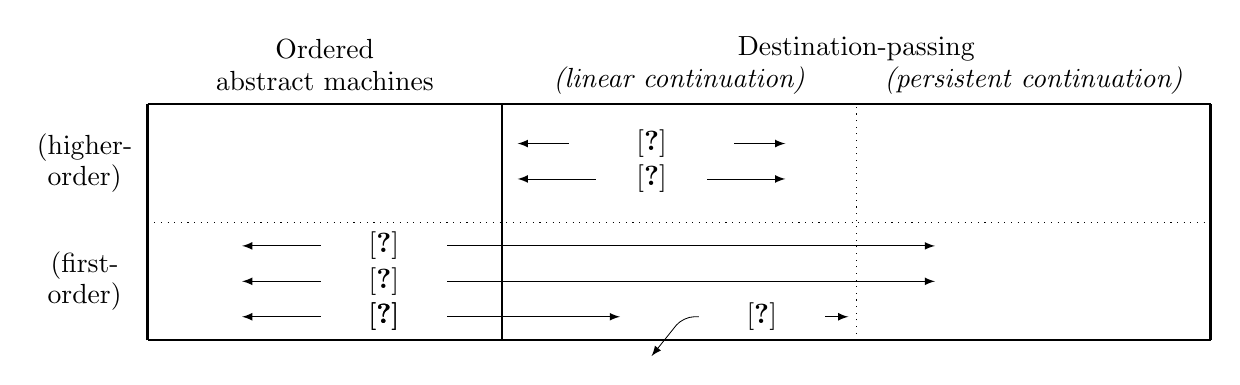
\begin{tikzpicture} 
\draw[thick](0cm,0cm) -- (0cm,3cm);
\draw (2.25,3.7) node{Ordered};
\draw (2.25,3.3) node{abstract machines};
%
\draw[thick](4.5cm,0cm) -- (4.5cm,3cm);
\draw (9,3.7) node{Destination-passing};
\draw (6.75,3.3) node{\it (linear continuation)};
%
\draw[dotted](9cm,0cm) -- (9cm,3cm);
\draw (11.25,3.3) node{\it (persistent continuation)};
%
\draw[thick](13.5cm,0cm) -- (13.5cm,3cm);
%
\draw[thick](0,0) -- (13.5,0);
\draw[dotted] (0,1.5) -- (13.5,1.5);
\draw[thick](0,3) -- (13.5,3);
%
\draw (-.8,2.45) node{(higher-};
\draw (-.8,2.05) node{order)};
%
\draw (-.8,0.95) node{(first-};
\draw (-.8,0.55) node{order)};
%
\draw (3,1.2) node{\cite{pfenning04substructural}};
\draw (3,.75) node{\cite{pfenning09substructural}};
\draw (3,.3) node{\cite{simmons11logical}};
\draw (3,.3) node{\cite{simmons11logical}};
\draw (7.8,.3) node{\cite{pfenning12substructural}};
\draw (6.4,2.5) node{\cite{cervesato02concurrent}};
\draw (6.4,2.05) node{\cite{schacknielsen07induction}};
%
\pgfsetarrowsstart{latex} 
\pgfsetlinewidth{.3pt} 
\pgfusepath{stroke} 
\draw (1.2,1.2) -- (2.2,1.2);
\draw (10,1.2) -- (3.8,1.2);
\draw (1.2,.75) -- (2.2,.75);
\draw (10,.75) -- (3.8,.75);
\draw (1.2,.3) -- (2.2,.3);
\draw (6,.3) -- (3.8,.3);
\draw[rounded corners=4pt] (6.4,-.2) -- (6.8,.3) -- (7,.3);
\draw (8.9,.3) -- (8.6,.3);
\draw (4.7,2.5) -- (5.35,2.5);
\draw (4.7,2.05) -- (5.7,2.05);
\draw (8.1,2.5) -- (7.45,2.5);
\draw (8.1,2.05) -- (7.1,2.05);
%
\end{tikzpicture} 
\end{center}
\caption{Classification of existing work on SSOS specifications}
\label{fig:class-prevwork}
\end{figure}


\noindent
The statement that each specification style is strictly more
expressive than the last is formal: by using fully automatic and
provably-correct transformations, natural semantics can be
mechanically transformed to ordered abstract machine semantics and
ordered abstract machine semantics can be mechanically transformed
into destination-passing semantics. These transformations are, in
turn, instances of general transformations on \sls~specifications.

\section{Logical correspondence}

\sls~is very
The potential design space of substructural operational semantics is
quite large. 

I propose that different styles of
\sls~specification can be productively classified in terms of the
transformations that turn one classification style into another. Most
transformations will not have inverses, so this methodology gives us a
formal notion of which styles are more expressive than others.
Considering logical transformations also can lower the cost of
mis-prediction. If one begins a development in an overly-restrictive
style, the development can be transformed into a more expressive style
by an automatic transformation.


\begin{center}
{\it Theme:}

\medskip

A logical framework based on forward reasoning in substructural logic
supports many styles of programming language specification. These
styles can be formally classified and connected by considering
generally applicable transformations on logical
specifications. Generally applicable transformations on logical
specifications are also useful for derive program analyses from those
operational semantics specifications.
\end{center}


